% Figures section: generated PNGs (scripts/paper-fig.py from paper/generated/fig-data.json, itself
% written by scripts/paper-fig-data.ts from bench/results/rq1-suite and bench/results/rq1-arm-k). \input
% this from wherever the Results section wants the figures (verifier/latex-build owner: place after the
% pass-rate and cost tables). Every number these figures draw is reused, never recomputed, from
% paper/tables/pass-rate-table.tex and paper/tables/cost-per-correct-table.tex, generated by
% scripts/paper-fig-tables.ts from the same fig-data.json.

\begin{figure}[t]
  \centering
  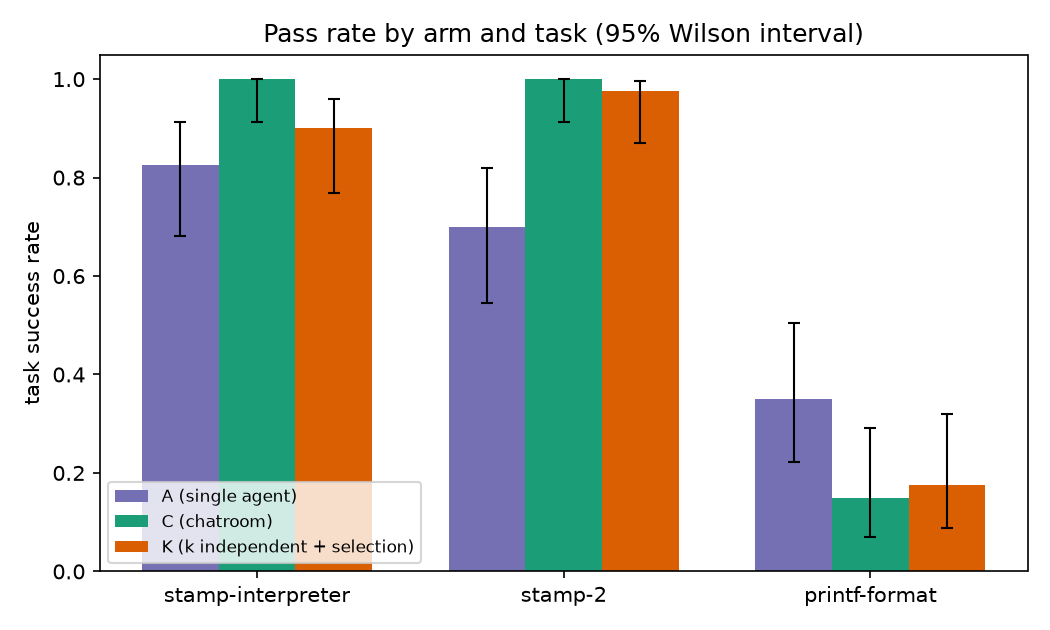
\includegraphics[width=\linewidth]{figures/fig-pass-rate.png}
  \caption{Task success rate by arm and task, with 95\% Wilson score intervals (n=40 seeds per cell).
  Arm C reaches ceiling on both interpreter-family tasks; on \texttt{bench-printf-format} both aggregation
  arms (C and K) fall below arm A, the negative case discussed in Section~\ref{sec:results}.}
  \label{fig:pass-rate}
\end{figure}

\begin{figure}[t]
  \centering
  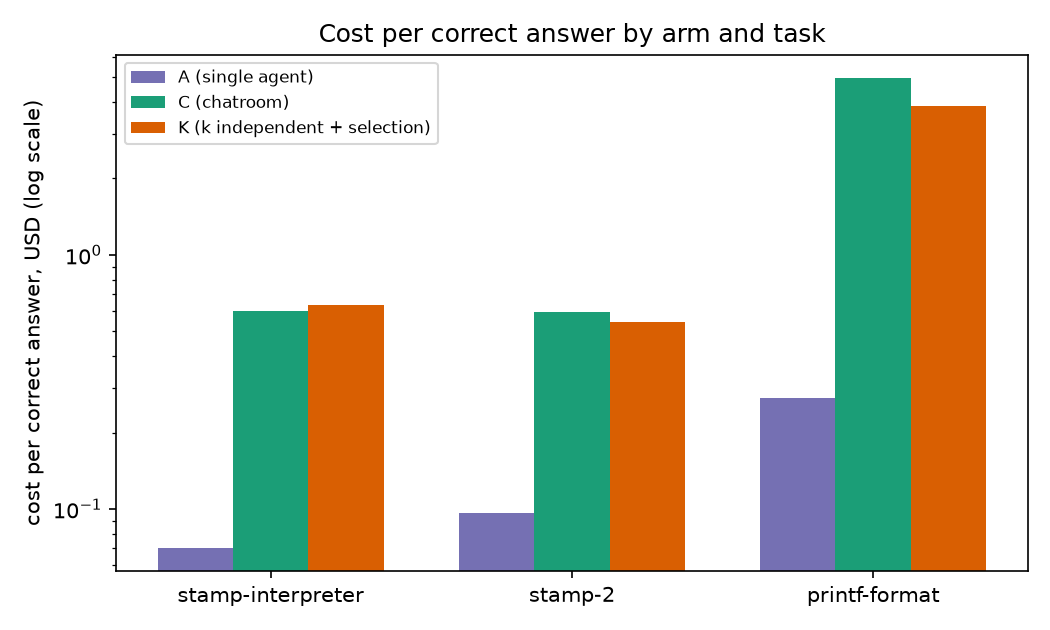
\includegraphics[width=\linewidth]{figures/fig-cost-per-correct.png}
  \caption{Cost per correct answer (API list price) by arm and task, log scale. Arm A is
  cheapest per correct answer on every task; arms C and K cost roughly the same as each other on the
  interpreter family and on \texttt{printf-format}, where both cost more per correct answer than arm A
  despite passing less often (Table~\ref{tab:cost-per-correct}). All runs are from before the thinking-budget
  regime shift documented in Section~\ref{sec:threats} (2026-09-19, 07:44--11:30 UTC); not comparable to any
  run from after the shift.}
  \label{fig:cost-per-correct}
\end{figure}

\begin{figure}[t]
  \centering
  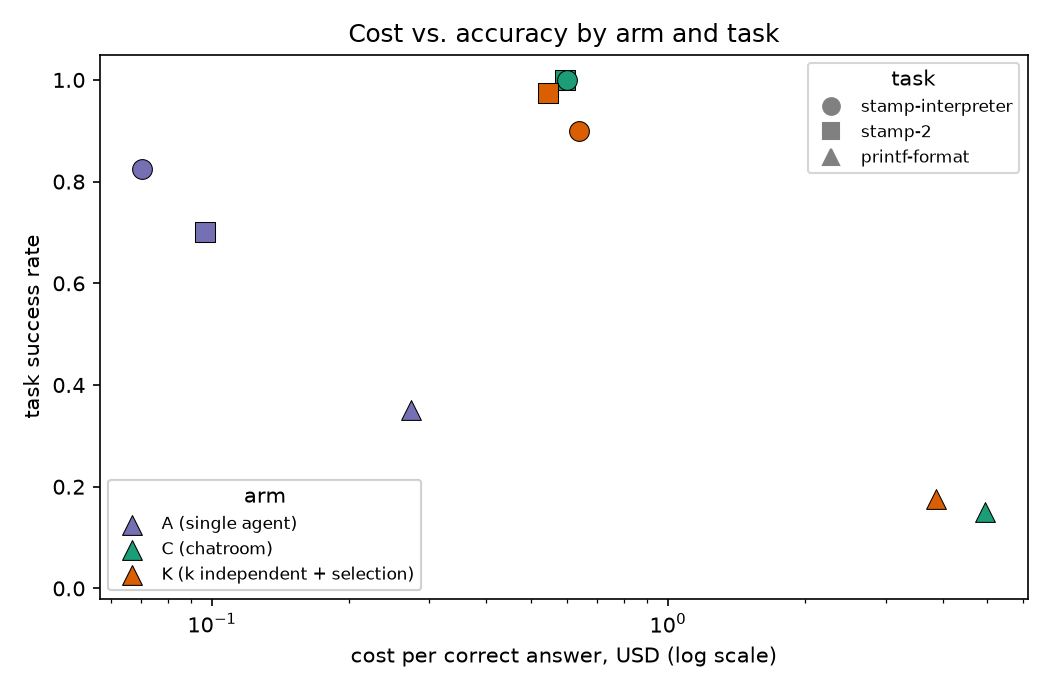
\includegraphics[width=\linewidth]{figures/fig-cost-vs-accuracy.png}
  \caption{Cost per correct answer (log scale) against task success rate, one point per (task, arm).
  Arm A is always cheapest per correct answer; arm C and arm K are budget-matched per prereg but neither
  buys accuracy on \texttt{printf-format}. All runs are from before the thinking-budget regime shift
  documented in Section~\ref{sec:threats} (2026-09-19, 07:44--11:30 UTC).}
  \label{fig:cost-vs-accuracy}
\end{figure}

\begin{figure}[t]
  \centering
  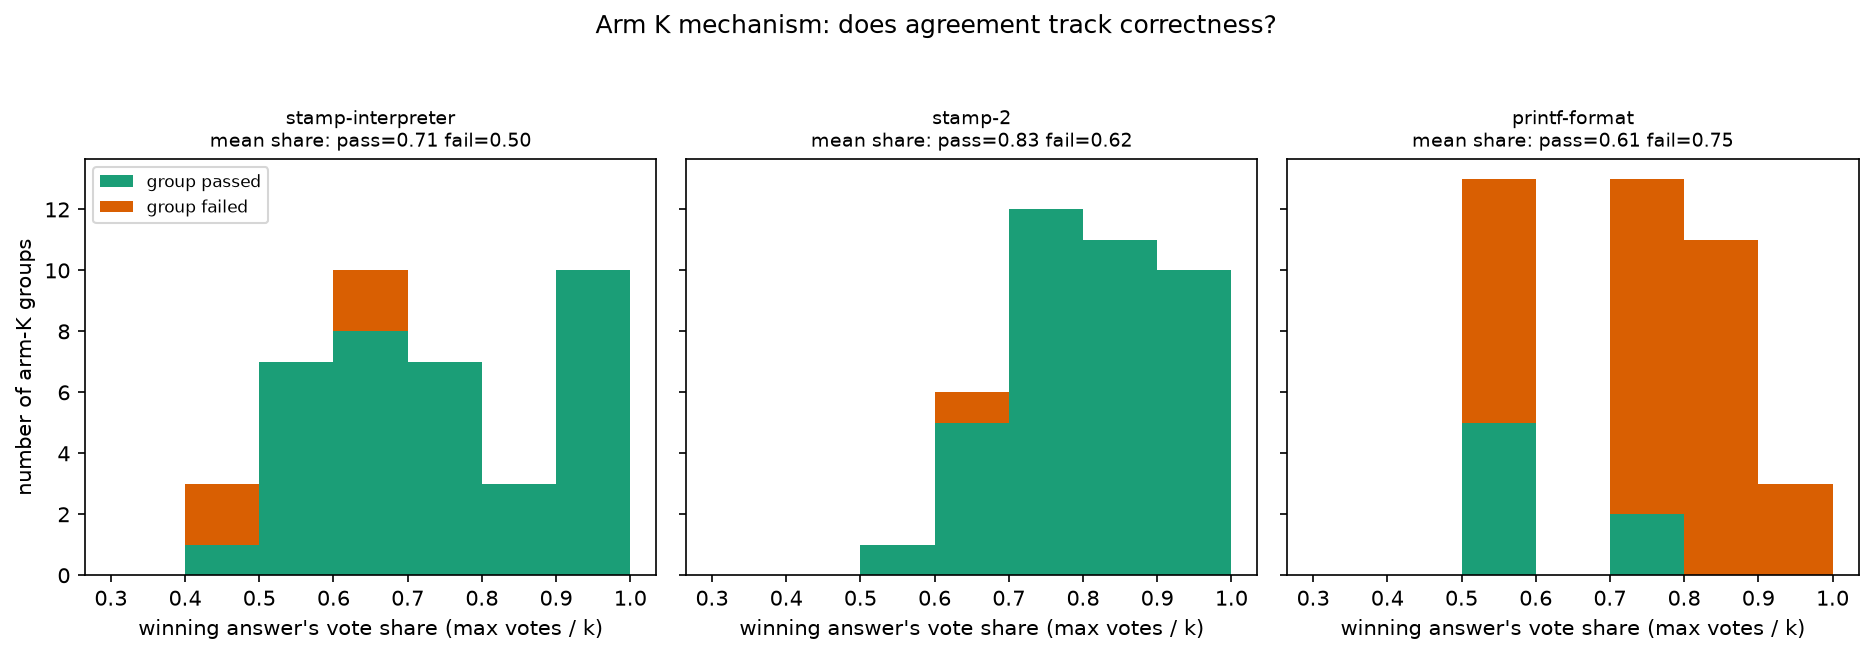
\includegraphics[width=\linewidth]{figures/fig-vote-mechanism.png}
  \caption{Mechanism figure: for every arm K group, the winning (plurality or MBR-exec) answer's vote
  share against whether the selected attempt passed the oracle. On the interpreter family a high vote
  share tracks passing (the shared wrong answer is a minority when it occurs at all); on
  \texttt{printf-format} a high vote share tracks \emph{failing} (the modal answer is the known
  \texttt{\%.17g} of \texttt{1e-07} defect, so both plurality and MBR-exec selection amplify the wrong
  cluster when it is the local majority). This is the empirical content behind
  paper/prereg-arm-k.md's prediction 2 and paper/amendments.md's printf selector calibration.}
  \label{fig:vote-mechanism}
\end{figure}
